\documentclass{standalone}

\begin{document}

\section[NLP]{Natural Language Processing}\label{chimera:nlp}

\begin{center}
\begin{figure}[htbp]
\centering
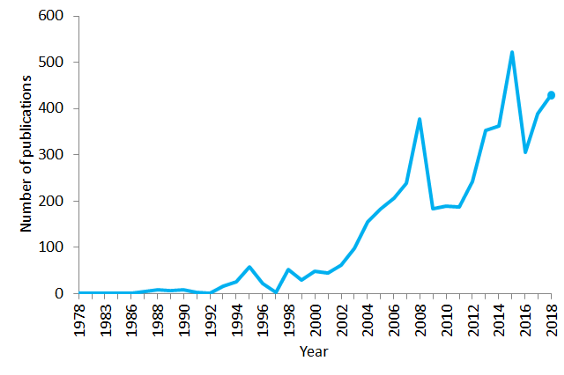
\includegraphics[width=\textwidth]{pubmed_nlp.png}
\caption{Number of publications containing the sentence \quotes{natural language processing} in PubMed in the period 1978–2018.
As of 2018, PubMed comprised more than 29 million citations for biomedical literature.
}
\label{fig:pubmed_nlp}
\end{figure}
\end{center}

Natural Language Processing (NLP) is a quite novel research field driven by the increasing availability of textual data (ref. Fig.~\ref{fig:pubmed_nlp}).
As told in the previous sections the incoming of Internet world exponentially increases the amount of data shared by people, and the major part of them are textual data, i.e data composed by words, phrases and, more in general, texts.
The NLP combines together techniques coming from linguistic, computer science, information theory and artificial intelligence researches.
It concerns the interactions between human languages and computers or, in other words, it studies how a computer can analyze a huge amount of natural language data, extracting numerical information from them.
This is a very hard task to perform since it is not straightforward to teach to a machine how humans communicate between them.
A key role is played by artificial intelligence researches which develop new algorithmic techniques to face these problems.

Most of the modern NLP techniques are based on a Machine Learning approach: thus we can find statistical methods and deep learning algorithms which aim to solve these tasks.
A first step to perform is the conversion of the human speech into a machine readable input; audio signals are so converted into string texts and only at this point the input can be analyzed from the machine.
Applying this work-flow in forward and reverse mode we can perform a communication between a human and machines, and vice versa.
In this section we will ignore how the conversion from human voice to numerical inputs could be performed and its related problems and solutions, focusing on the latest part of this pipeline, i.e in the description of the common techniques used to convert a string text into numeric values.
This is also the case related to our \textsf{CHIMeRA} project, in which we have a huge amount of names and strings associated to medical terms and we want to standardize them increasing their overlap.

First of all, we have to take care that each human language has its own characteristics and thus it is hard to create a pipeline ables to process all the languages at the same time, while it is easier to tune an algorithm on a particular language.
In our work we focused on Italian (\textsf{SymptomsNet}) and English (\textsf{CHIMeRA} Network) languages.
Since \textsf{SymptomsNet} project has been developed as simple proof of concepts, the developed Italian pipeline was really naive and, for sake of brevity, we will focus only on the \textsf{CHIMeRA} pipeline, i.e the English one.
We would stress that in our application we are not interested on the understanding of words meaning, but we want to minimize the word heterogeneity, maximizing their overlap.
Thus, we have ignored the semantic strings meaning and we have focused only on their syntaxes.

The syntax is the set of rules, principles and processes that govern the structure of sentences in a given language.
We can create groups of words applying grammatical rules: grammatical rules have to be converted into algorithms which take in input a word and give in output a processed version of it.
In this case there is not a numerical output, but just a reorganization of string letters and words.
The most common techniques involved in syntactic analysis are:

\begin{itemize}

  \item \textbf{Sentence breaking:} it divides a continuous text into sentences placing boundaries.
  \item \textbf{Word segmentation (tokenization):} it splits a large set of continuous text into units.
  \item \textbf{Parsing:} it provides the grammatical analysis of the provided sentence.
  \item \textbf{Morphological segmentation:} it splits words into individual units called morphemes.
  \item \textbf{Part-of-speech tagging:} it finds the grammatical parts of speech for every word.
  \item \textbf{Lemmatization:} it reduces the inflectional forms of a word into a single form.
  \item \textbf{Stemming:} it cuts the inflected words to their root form.

\end{itemize}

All these algorithms are very similar each other, so to better understand their functionality is useful an example.
Let start from a useless text taken from the NLP \href{https://en.wikipedia.org/wiki/Natural_language_processing}{Wikipedia} web-page:

\lstset{style=snippet}
\begin{lstlisting}[language=Python, caption=Original text, label=code:orig]
text = "Natural language processing (NLP) is a subfield of linguistics, computer science, information engineering, and artificial intelligence concerned with the interactions between computers and human (natural) languages, in particular how to program computers to process and analyze large amounts of natural language data. Challenges in natural language processing frequently involve speech recognition, natural language understanding, and natural language generation."
\end{lstlisting}

First of all we notice that the text is made by two sentences, that can be broken using a \emph{sentence breaking} algorithm.
In this way, we obtain a list of two strings given by

\lstset{style=snippet}
\begin{lstlisting}[language=Python, caption=Sentence breaking, label=code:sentence]
sentence_1 = "Natural language processing (NLP) is a subfield of linguistics, computer science, information engineering, and artificial intelligence concerned with the interactions between computers and human (natural) languages, in particular how to program computers to process and analyze large amounts of natural language data."

sentence_2 = "Challenges in natural language processing frequently involve speech recognition, natural language understanding, and natural language generation."
\end{lstlisting}

Now, we can divide each sentence into its set of words, using a word \emph{tokenization}.
Focusing only on the first sentence, we obtain in output:

\lstset{style=snippet}
\begin{lstlisting}[language=Python, caption=Tokenization, label=code:token]
tokens = ['Natural', 'language', 'processing', '(', 'NLP', ')', 'is', 'a', 'subfield', 'of', 'linguistics', ',', 'computer', 'science', ',', 'information', 'engineering', ',', 'and', 'artificial', 'intelligence', 'concerned', 'with', 'the', 'interactions', 'between', 'computers', 'and', 'human', '(', 'natural', ')', 'languages', ',', 'in', 'particular', 'how', 'to', 'program', 'computers', 'to', 'process', 'and', 'analyze', 'large', 'amounts', 'of', 'natural', 'language', 'data', '.']
\end{lstlisting}

There are multiple useless tokens in the processed list and we can filter them using a type of \emph{part-of-speech tagging} algorithm, which removes the so-called \emph{stop words} and punctuations.
In our example our list of tokens becomes

\lstset{style=snippet}
\begin{lstlisting}[language=Python, caption=Filtering stop-words and punctuations, label=code:filter]
tokens = ['Natural', 'language', 'processing', 'NLP', 'subfield', 'linguistics', 'computer', 'science', 'information', 'engineering', 'artificial', 'intelligence', 'concerned', 'interactions', 'computers','human', 'natural', 'languages', 'particular', 'program', 'computers', 'process', 'analyze', 'large', 'amounts', 'natural', 'language', 'data']
\end{lstlisting}

A final processing could be given by a \emph{stemming} algorithm, which extracts the root form of each word.
Using a stemmer on the previous set of words we obtain

\lstset{style=snippet}
\begin{lstlisting}[language=Python, caption=Stemming, label=code:stem]
tokens = ['natur', 'languag', 'process', 'nlp', 'subfield', 'linguist', 'comput', 'scienc', 'inform', 'engin', 'artifici', 'intellig', 'concern', 'interact', 'comput', 'human', 'natur', 'languag', 'particular', 'program', 'comput', 'process', 'analyz', 'larg', 'amount', 'natur', 'languag', 'data']
\end{lstlisting}

As can be seen by this example, the stemming algorithm converts in lower case each letter of each word and it removes the inflections from each of them.
This is a very naive example, but we can already notice as our processing allows to merge multiple words together.
In the original sentence we have the word \quotes{\emph{Natural}} (with capital letter) and two occurrences of \quotes{\emph{natural}} (lower case).
Moreover, we have three occurrences of the \quotes{\emph{computer}} word, but only two of them are in singular form.
The \textsf{tokenization + stemming} processing allows to compare different word forms making them compatible.

Combinations of these algorithms can be found in everyday applications, starting from email assistants or website chat box, to the more advanced sentiment analyses and fake news identifiers~\cite{IJST119594, MitaliSentiment2016, sharma2019combating, zhou2018fake}.
NLP pipelines are used also in biomedical applications and modern multinational companies like Amazon, IBM or Google are financing different kinds of research on this topic.
\href{https://aws.amazon.com/it/comprehend/medical/}{Amazon Comprehend Medical} is a NLP service developed by Amazon to extract disease conditions, medications and treatment outcomes from patient notes, electronic health records and other clinical trial reports.
At the same time, also companies like Yahoo and Google base their filters and email classifiers on NLP algorithms to stop email-spam.
Also the hot topic of these last years about the fake news is faced using NLP pipelines and the NLP Group at MIT is developing new tools to determine if a source is accurate or politically biased based on text analyses.

In our applications we built a custom pipeline based on a part of the described above functions.
In the following sections we will describe in detail our pipeline: we would stress that the efficiency of our pipeline could not be generalized to other datasets, since our purpose was to obtain the best result for our application.
In other words, we had fine-tuned our pipeline based on the data used in this project.
Moreover, we have to clarify that our pipeline is not fully-automatic, but it was made according to a semi-supervised approach: we customized the work-flow following the encountered issues.


\end{document}
